\documentclass[10pt,letterpaper]{article}

\usepackage[margin=0.62in,headheight=16pt,footskip=24pt]{geometry}
\usepackage[T1]{fontenc}
\usepackage{helvet}
\renewcommand{\familydefault}{\sfdefault}
\usepackage{graphicx}
\usepackage{array,tabularx}
\usepackage{enumitem}
\usepackage{xcolor}
\usepackage{fancyhdr}
\usepackage[hidelinks]{hyperref}

\definecolor{Navy}{HTML}{173B63}
\definecolor{Blue}{HTML}{1F6FB2}
\definecolor{Pale}{HTML}{EAF2F8}
\definecolor{Ink}{HTML}{1D2733}
\definecolor{Muted}{HTML}{5C6875}
\definecolor{Line}{HTML}{CAD6E2}

\hypersetup{
  colorlinks=true,
  urlcolor=Blue,
  linkcolor=Blue,
  pdfauthor={Vo Hong Quan},
  pdftitle={Technical Portfolio — Vo Hong Quan},
  pdfsubject={Reinforcement learning for robot control}
}

\setlength{\parindent}{0pt}
\setlength{\parskip}{4pt}
\setlist[itemize]{leftmargin=1.2em,itemsep=2pt,topsep=3pt,parsep=0pt}
\urlstyle{same}

\newcommand{\PortfolioUrl}{https://vohongquann.github.io/Portfolio}
\newcommand{\PortfolioText}{vohongquann.github.io/Portfolio}
\newcommand{\Email}{vohongquan.6524@gmail.com}
\newcommand{\GithubUrl}{https://github.com/vohongquann}
\newcommand{\GithubText}{github.com/vohongquann}
% Single source of truth for project facts shared by the CV and portfolio.
% Keep portfolio-only architecture, images and limitations in portfolio.tex.

\newcommand{\crazyTitle}{Crazyflie-IsaacLab: RL-Tuned PID Gains for a Crazyflie Quadrotor}
\newcommand{\crazyTech}{Python, PyTorch, PPO (rsl\_rl), NVIDIA Isaac Lab}
\newcommand{\crazyUrl}{https://github.com/vohongquann/Crazyflie-IsaacLab}
\newcommand{\crazyLinkText}{github.com/vohongquann/Crazyflie-IsaacLab}
\newcommand{\crazyDate}{Jan 2026 -- Sep 2026}
\newcommand{\crazyBulletOne}{Built a four-layer flight controller (50--500 Hz) and physics-based Crazyflie model in Isaac Lab 3.0.}
\newcommand{\crazyBulletTwo}{Trained one PPO MLP per layer to tune 9 PID gains, reducing tracking error 23--62\% versus PID (attitude: 15.5\textdegree{} to 5.9\textdegree{}).}
\newcommand{\crazyBulletThree}{Anchored zero network output to the stable PID baseline and sized each MLP for STM32 deployment.}

\newcommand{\balanceTitle}{BalancingRobot-IsaacLab: Self-Balancing Robot with an RL Cascade}
\newcommand{\balanceTech}{Python, PPO (rsl\_rl), ROS 2, ONNX, LQR, PID}
\newcommand{\balanceUrl}{https://github.com/vohongquann/BalancingRobot-IsaacLab}
\newcommand{\balanceLinkText}{github.com/vohongquann/BalancingRobot-IsaacLab}
\newcommand{\balanceDate}{Jun 2025 -- Dec 2025}
\newcommand{\balanceBulletOne}{Trained a PPO velocity policy that maps commands and raw IMU/encoder data to wheel torques.}
\newcommand{\balanceBulletTwo}{Added a frozen position policy; recorded zero falls in 768 randomized episodes and 8 mm median goal error.}
\newcommand{\balanceBulletThree}{Beat LQR on speed steps: 0.026 m/s error in 0.36 s versus 0.067 m/s in 1.1 s.}

\newcommand{\rotaryTitle}{RotaryPendulum-IsaacLab: Learned Cascade PID for a Rotary Inverted Pendulum}
\newcommand{\rotaryTech}{Python, PPO (rsl\_rl), NVIDIA Isaac Lab, PhysX, URDF}
\newcommand{\rotaryUrl}{https://github.com/vohongquann/RotaryPendulum-IsaacLab}
\newcommand{\rotaryLinkText}{github.com/vohongquann/RotaryPendulum-IsaacLab}
\newcommand{\rotaryDate}{Feb 2025 -- May 2025}
\newcommand{\rotaryBulletOne}{Modeled the QUBE-Servo 2 from CAD with a DC motor and quantized encoders at 500 Hz.}
\newcommand{\rotaryBulletTwo}{Trained a PPO policy on 4,096 robots in 64 minutes to tune six cascade-PID gains at 100 Hz.}
\newcommand{\rotaryBulletThree}{Validated on 256 randomized robots: 0.40 s swing-up, 0.23--0.50 s settling and at most 1.4\textdegree{} median overshoot.}


\pagestyle{fancy}
\fancyhf{}
\fancyhead[L]{\small\bfseries\color{Navy} VO HONG QUAN}
\fancyhead[R]{\small\color{Muted} TECHNICAL PORTFOLIO}
\fancyfoot[L]{\footnotesize\href{mailto:\Email}{\Email}}
\fancyfoot[C]{\footnotesize\href{\PortfolioUrl}{\PortfolioText}}
\fancyfoot[R]{\footnotesize\color{Muted}\thepage}
\renewcommand{\headrulewidth}{0.4pt}
\renewcommand{\footrulewidth}{0pt}

\newcommand{\PageTitle}[2]{%
  {\footnotesize\bfseries\color{Blue}#1}\par
  {\raggedright\fontsize{19}{22}\selectfont\bfseries\color{Navy}#2\par}
  \vspace{2pt}\color{Line}\rule{\linewidth}{0.8pt}\color{Ink}\vspace{5pt}
}

\newcommand{\Label}[1]{{\footnotesize\bfseries\color{Blue}#1}\par}
\newcommand{\MiniTitle}[1]{{\large\bfseries\color{Navy}#1}\par}

\newcommand{\Contact}[2]{%
  \colorbox{Pale}{\parbox[c][0.58in][c]{0.44\linewidth}{%
    \Label{#1}\small #2}}
}

\newcommand{\SkillBox}[2]{%
  \parbox[t]{0.47\linewidth}{\Label{#1}\small #2}
}

\newcommand{\Metric}[2]{%
  \colorbox{Pale}{\parbox[c][0.78in][c]{0.285\linewidth}{%
    \centering{\fontsize{17}{19}\selectfont\bfseries\color{Navy}#1}\par
    \footnotesize\color{Muted}#2}}
}

\newcommand{\ProjectMeta}[4]{%
  \renewcommand{\arraystretch}{1.22}%
  \begin{tabularx}{\linewidth}{@{}>{\bfseries\color{Blue}}p{0.13\linewidth}X>{\bfseries\color{Blue}}p{0.13\linewidth}X@{}}
    ROLE & #1 & PERIOD & #2\\
    DOMAIN & #3 & REPOSITORY & #4
  \end{tabularx}
  \renewcommand{\arraystretch}{1}
}

\begin{document}
\color{Ink}

% Cover -------------------------------------------------------------------
\thispagestyle{empty}
\vspace*{0.4in}
{\small\bfseries\color{Blue} TECHNICAL PORTFOLIO \hfill 2026}\par
\vspace{0.7in}
{\fontsize{34}{38}\selectfont\bfseries\color{Navy}Vo Hong Quan}\par
\vspace{0.12in}
{\fontsize{19}{23}\selectfont\color{Blue}Reinforcement Learning for Robot Control}\par
\vspace{0.25in}
{\large\color{Muted}Models, trains and benchmarks learning-based controllers in simulation.}\par
\vspace{0.45in}
\color{Line}\rule{\linewidth}{1pt}\color{Ink}
\vspace{0.35in}

\Contact{EMAIL}{\href{mailto:\Email}{\Email}}\hfill
\Contact{PHONE}{\href{tel:+84363645485}{(+84) 363 645 485}}\par\vspace{0.18in}
\Contact{GITHUB}{\href{\GithubUrl}{\GithubText}}\hfill
\Contact{WEBSITE}{\href{\PortfolioUrl}{\PortfolioText}}

\vfill
\begin{minipage}[b]{0.72\linewidth}
  \Label{FOCUS}
  Reinforcement learning · cascaded control · robotics simulation · embedded deployment

  \vspace{0.2in}
  \small Every contact, repository and project title in this PDF is clickable.
\end{minipage}
\hfill
\begin{minipage}[b]{0.18\linewidth}
  \centering
  \href{\PortfolioUrl}{
\includegraphics[width=0.92\linewidth]{assets/portfolio/portfolio-qr.png}}\\[-1pt]
  {\scriptsize\color{Muted}Open portfolio}
\end{minipage}
\vspace*{0.25in}

% Profile -----------------------------------------------------------------
\newpage
\PageTitle{01 · PROFILE}{Profile \& Background}

\MiniTitle{Professional profile}
Robotics and AI engineer focused on learning-based control. Builds physical models, trains reinforcement learning policies and compares them with PID and LQR baselines. Seeking an AI or robotics engineering internship that connects simulation with real hardware.

\vspace{0.15in}
\MiniTitle{Core expertise}
\vspace{4pt}
\SkillBox{REINFORCEMENT LEARNING}{PPO, SAC, reward design, hyperparameter tuning, frozen policy cascades}
\hfill
\SkillBox{CONTROL SYSTEMS}{Cascaded PID, LQR, motor and sensor modeling, step-response analysis}\par\vspace{0.16in}
\SkillBox{ROBOTICS \& SIMULATION}{NVIDIA Isaac Sim and Isaac Lab, PhysX, ROS 2, URDF from CAD}
\hfill
\SkillBox{ML \& VISION}{PyTorch, TensorFlow, Keras, scikit-learn, OpenCV, YOLO}\par\vspace{0.16in}
\SkillBox{PROGRAMMING}{Python, C/C++, MATLAB, Git, Linux, pytest}
\hfill
\SkillBox{DEPLOYMENT \& EVALUATION}{ONNX, ESP32, STM32-sized networks, randomized tests and reproducible scripts}

\vspace{0.28in}
\colorbox{Pale}{\parbox{0.965\linewidth}{%
  \vspace{5pt}
  \Label{EXPERIENCE}
  \textbf{Research Assistant — Robotics Lab, Ho Chi Minh City University of Technology and Engineering}\hfill Feb 2025--Present
  \begin{itemize}
    \item Train and evaluate reinforcement learning controllers for real-time robotic systems.
    \item Design reward functions and tune hyperparameters for stable policies.
  \end{itemize}
  \vspace{2pt}
  \Label{EDUCATION}
  \textbf{Bachelor of Robotics and Artificial Intelligence}\hfill Expected Dec 2026\\
  Ho Chi Minh City University of Technology and Engineering · GPA 3.22/4.0
  \vspace{4pt}
}}

\vspace{0.23in}
\begin{tabularx}{\linewidth}{@{}>{\bfseries\color{Blue}}p{0.19\linewidth}X@{}}
  CERTIFICATION & TOEIC Listening \& Reading 715/990, IIG Vietnam (2025)\\[3pt]
  LANGUAGES & Vietnamese (native); English (TOEIC 715/990)
\end{tabularx}

% Crazyflie ---------------------------------------------------------------
\newpage
\PageTitle{02 · CASE STUDY}{\crazyTitle}
Small PPO networks tune each layer of a four-loop flight controller for a Crazyflie 2.1 Brushless.

\vspace{5pt}
\ProjectMeta{Individual: model, train, evaluate}{\crazyDate}{\crazyTech}{\href{\crazyUrl}{Open GitHub}}

\vspace{0.12in}
\href{\crazyUrl}{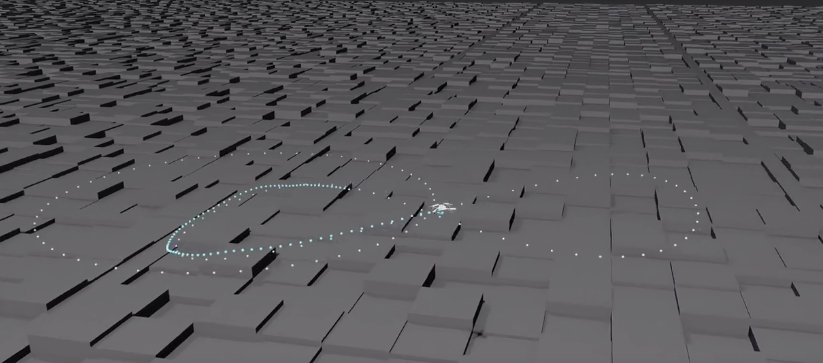
\includegraphics[width=\linewidth,height=2.05in,keepaspectratio]{assets/portfolio/crazyflie.png}}

\begin{minipage}[t]{0.47\linewidth}
  \Label{ENGINEERING PROBLEM}
  Track position commands through position, velocity, attitude and rate loops running at 50--500 Hz, with networks small enough for the drone's STM32.
\end{minipage}
\hfill
\begin{minipage}[t]{0.49\linewidth}
  \Label{CONTRIBUTION}
  \begin{itemize}
    \item \crazyBulletOne
    \item \crazyBulletTwo
    \item \crazyBulletThree
  \end{itemize}
\end{minipage}

\vspace{0.12in}
\colorbox{Pale}{\parbox{0.965\linewidth}{%
  \Label{SYSTEM FLOW}
  Position 50 Hz $\rightarrow$ velocity 100 Hz $\rightarrow$ attitude 250 Hz $\rightarrow$ rate 500 Hz $\rightarrow$ motors\\
  Each small MLP maps observations to 9 PID gains; zero output recovers the stable PID baseline.
}}

\vspace{0.16in}
\Metric{23--62\%}{lower tracking error across all four layers}\hfill
\Metric{15.5\textdegree{} $\to$ 5.9\textdegree{}}{attitude error, PID to RL gains}\hfill
\Metric{2.6--6.3$\times$}{outer-loop motor chatter; next improvement}

% Balancing robot ---------------------------------------------------------
\newpage
\PageTitle{03 · CASE STUDY}{\balanceTitle}
A velocity policy balances a Pololu Balboa; a frozen position policy drives it to a goal.

\vspace{5pt}
\ProjectMeta{Individual: model, train, ROS 2}{\balanceDate}{\balanceTech}{\href{\balanceUrl}{Open GitHub}}

\vspace{0.12in}
\href{\balanceUrl}{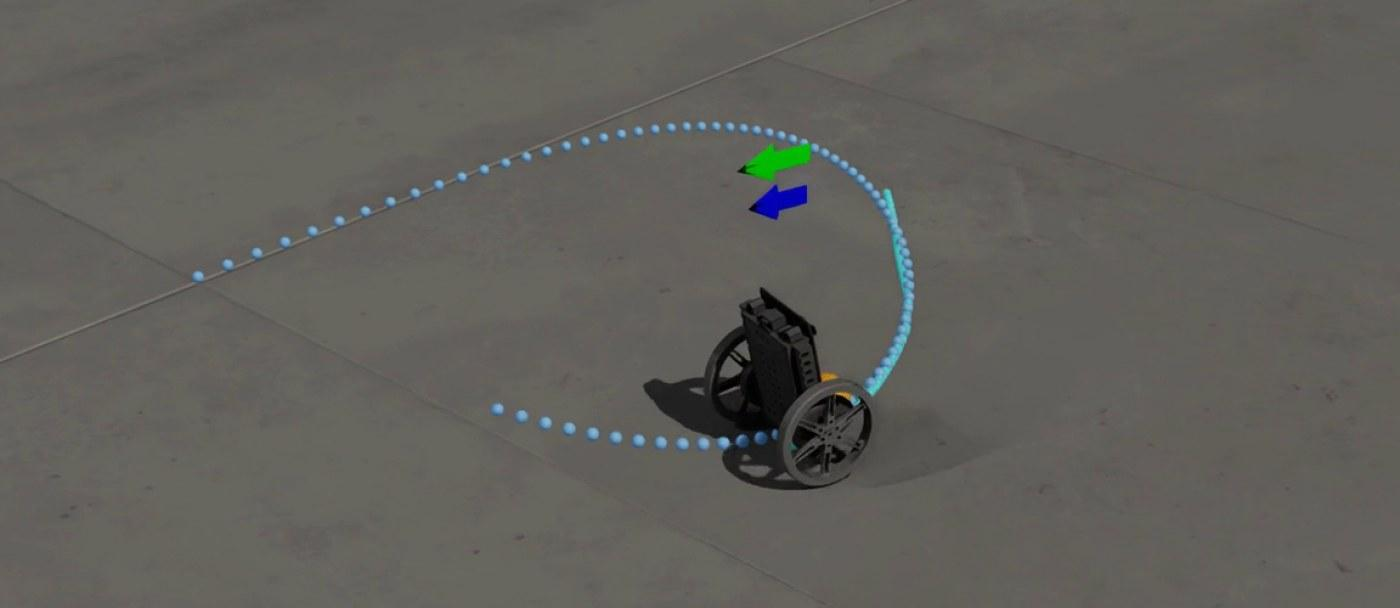
\includegraphics[width=\linewidth,height=2.05in,keepaspectratio]{assets/portfolio/balancing-robot.jpg}}

\begin{minipage}[t]{0.47\linewidth}
  \Label{ENGINEERING PROBLEM}
  Balance and navigate using only a noisy IMU and wheel encoders while tolerating pushes and changes in mass, friction and center of mass.
\end{minipage}
\hfill
\begin{minipage}[t]{0.49\linewidth}
  \Label{CONTRIBUTION}
  \begin{itemize}
    \item \balanceBulletOne
    \item \balanceBulletTwo
    \item \balanceBulletThree
  \end{itemize}
\end{minipage}

\vspace{0.12in}
\colorbox{Pale}{\parbox{0.965\linewidth}{%
  \Label{SYSTEM FLOW}
  IMU + encoders $\rightarrow$ complementary filter $\rightarrow$ position policy $\rightarrow$ frozen velocity policy $\rightarrow$ wheel torque\\
  Evaluated over 768 episodes with pushes, sensor noise and randomized dynamics.
}}

\vspace{0.16in}
\Metric{0 falls}{in 768 randomized episodes}\hfill
\Metric{8 mm}{median goal-position error}\hfill
\Metric{0.36 s}{speed-step settling; LQR: 1.1 s}

% Rotary pendulum ---------------------------------------------------------
\newpage
\PageTitle{04 · CASE STUDY}{\rotaryTitle}
A PPO policy retunes both loops of a QUBE-Servo 2 cascade PID at 100 Hz.

\vspace{5pt}
\ProjectMeta{Individual: model, train, evaluate}{\rotaryDate}{\rotaryTech}{\href{\rotaryUrl}{Open GitHub}}

\vspace{0.12in}
\href{\rotaryUrl}{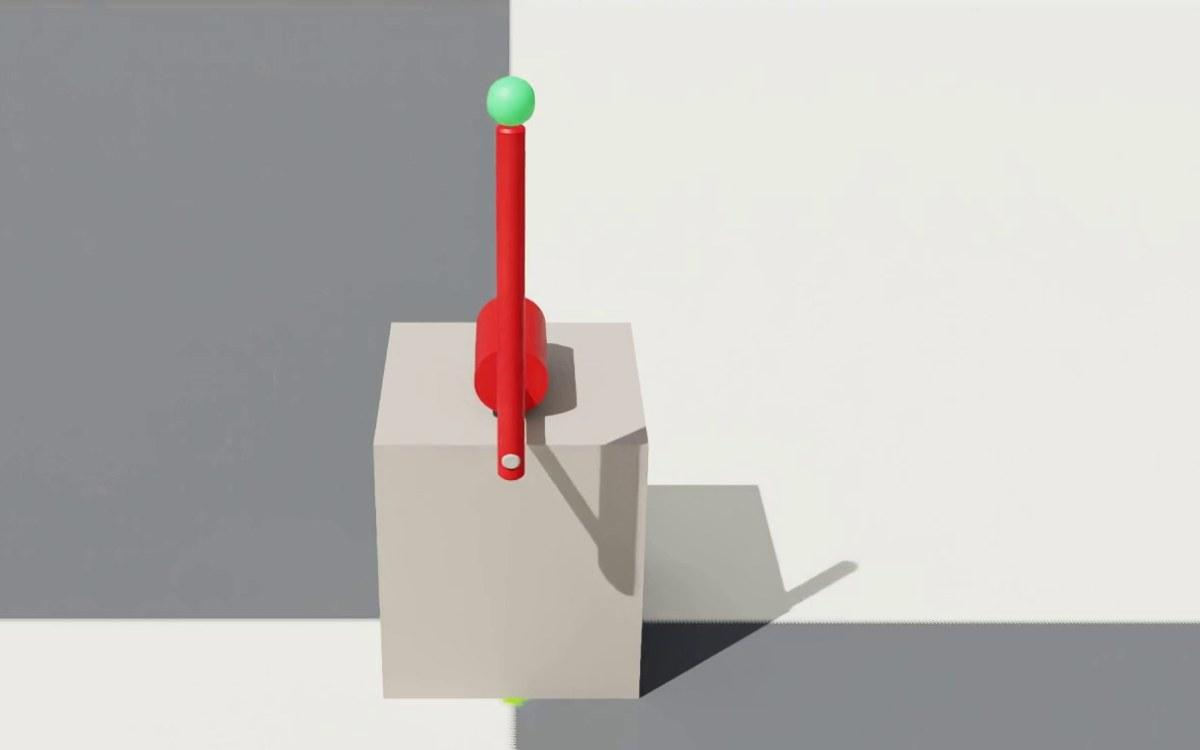
\includegraphics[width=\linewidth,height=2.05in,keepaspectratio]{assets/portfolio/rotary-pendulum.jpg}}

\begin{minipage}[t]{0.47\linewidth}
  \Label{ENGINEERING PROBLEM}
  Swing up and balance the pendulum while tracking arm-angle commands despite quantized encoders and varied motor constants.
\end{minipage}
\hfill
\begin{minipage}[t]{0.49\linewidth}
  \Label{CONTRIBUTION}
  \begin{itemize}
    \item \rotaryBulletOne
    \item \rotaryBulletTwo
    \item \rotaryBulletThree
  \end{itemize}
\end{minipage}

\vspace{0.12in}
\colorbox{Pale}{\parbox{0.965\linewidth}{%
  \Label{SYSTEM FLOW}
  12 observations $\rightarrow$ PPO at 100 Hz $\rightarrow$ 6 gains $\rightarrow$ outer PID 250 Hz $\rightarrow$ inner PID 500 Hz\\
  Evaluated on 256 robots, each with randomized motor constants.
}}

\vspace{0.16in}
\Metric{0.40 s}{median swing-up time}\hfill
\Metric{0.23--0.50 s}{median arm-step settling}\hfill
\Metric{$\leq$ 1.4\textdegree{}}{median overshoot; $\leq$ 0.24\textdegree{} steady error}

\end{document}
